A figura \ref{figura:ciclo}, retirada dos slides de aula, mostra o ciclo de um item de configuração. Ele fica, inicialmente, armazenado no repositório de itens de configuração que, na nomenclatura do \textit{Github}, é chamado simplesmente de repositório ou \textit{repository}.
\par As ramificações de projeto, citadas em aula, são equivalentes aos \textit{branches} no \textit{Github}. Um item de configuração que foi revisado e está armazenado em um repositório - item de configuração \textit{baselined} - é conhecido como um arquivo \textit{tracked}.
\begin{figure}[H]
    \caption{Ilustração do ciclo de um item de configuração}
    \vspace{0.5cm}
    \centering
    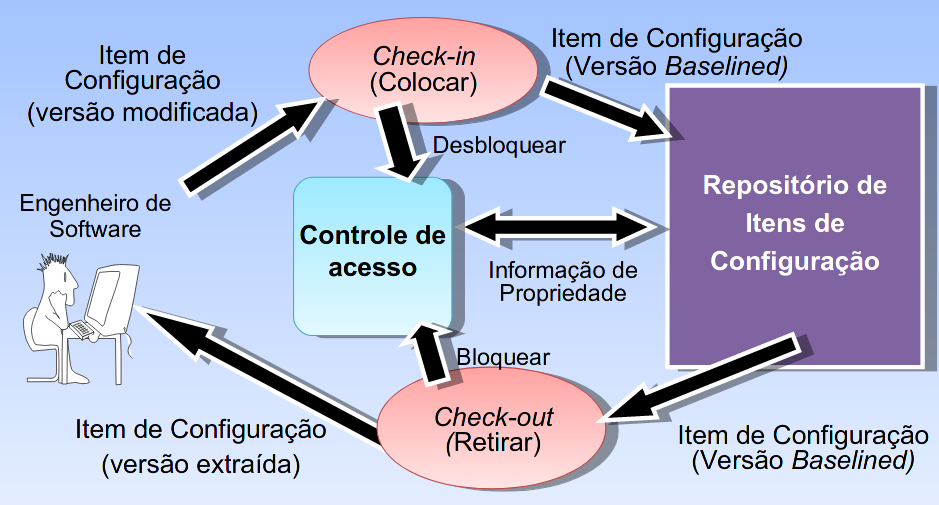
\includegraphics[width=15cm]{imagens/ciclo_gerenciamento.png}
    \label{figura:ciclo}
\end{figure}

\par Para retirar um item de configuração na versão em que está armazenado no repositório, é necessário realizar um \textit{check-out}. Isso é o equivalente a clonar um repositório - \textit{git clone} - para a ocasião em que o repositório apenas exista remotamente ou a realizar um \textit{git fetch} seguido de um \textit{git pull} quando o repositório já existe localmente mas não tem todas as atualizações do repositório remoto.
\par A versão extraída, então, é submetida a mudanças e passa a ser um arquivo modificado rastreado - \textit{tracked} - pelo \textit{Git}. O usuário realiza as modificações e o item de configuração se torna uma versão modificada ou \textit{modified}.
\par Caso deseje realizar o \textit{check-in} das modificações, são necessários dois passos. O primeiro consiste em utilizar o comando \textit{git add} seguido pelo comando \textit{git commit}. Eles são responsáveis, respectivamente, por adicionar os itens de configuração modificados para a área de \textit{stage} (área composta pelos arquivos que farão parte do próximo \textit{commit}) e por salvar as mudanças em uma nova versão, inicialmente apenas no repositório local.
\par Em seguida, ainda é preciso atualizar o repositório remoto com as modificações. Caso o usuário que modificou seja dono do repositório e esteja trabalhando no mesmo \textit{branch} que deseja modificar, basta usar o comando \textit{git push}. Por outro lado, caso se trate de um colaborador trabalhando na sua cópia do projeto, é preciso realizar um \textit{pull request}.

\begin{figure}[H]
    \caption{Ciclo de estados de item de configuração no \textit{Git}}
    \vspace{0.5cm}
    \centering
    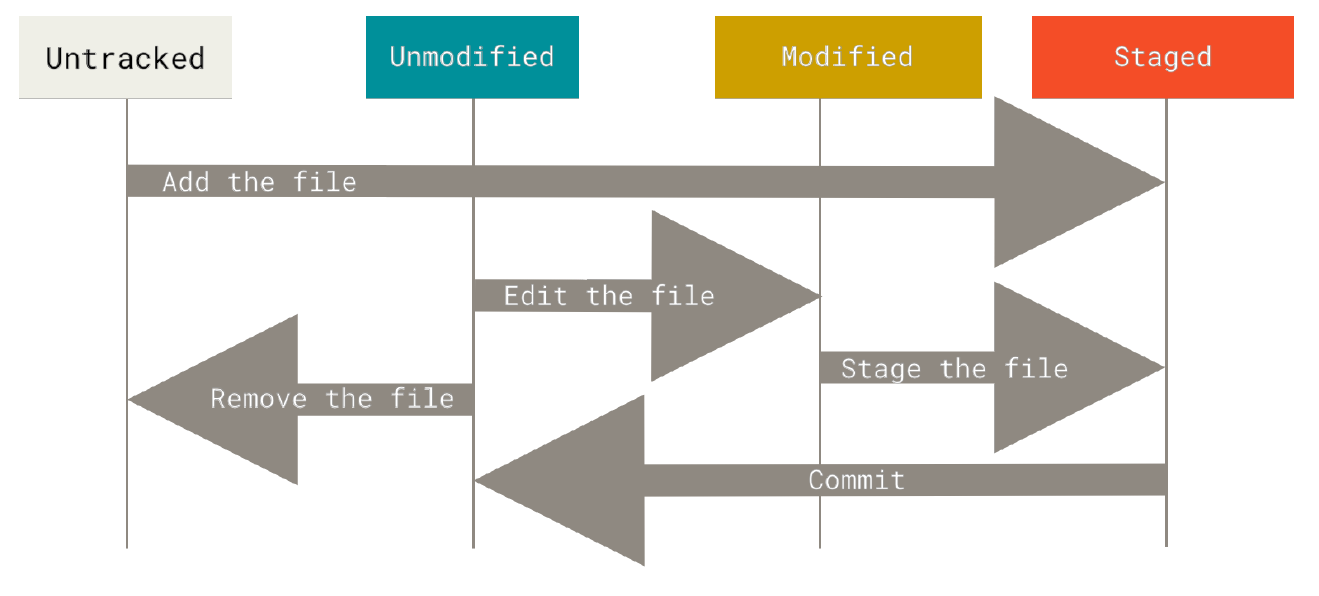
\includegraphics[width=15cm]{imagens/ciclo_estados.png}
    \label{figura:ciclo_estados}
\end{figure}

A figura \ref{figura:ciclo_estados} foi retirada do livro \href{https://git-scm.com/book/en/v2}{\textit{ProGit}} e ilustra o ciclo de um item de configuração gerenciado com \textit{Git}.
Nela, é exibido apenas o ciclo local de item de configuração.
\par A figura \ref{figura:secoes_projeto_git}, por outro lado, exibe a dinâmica de \textit{check-in} e \textit{check-out} de um projeto gerenciado por \textit{Git}. Ela também foi retirada do livro \href{https://git-scm.com/book/en/v2}{\textit{ProGit}}.

\begin{figure}[H]
    \caption{Ciclo de estados de item de configuração no \textit{Git}}
    \vspace{0.5cm}
    \centering
    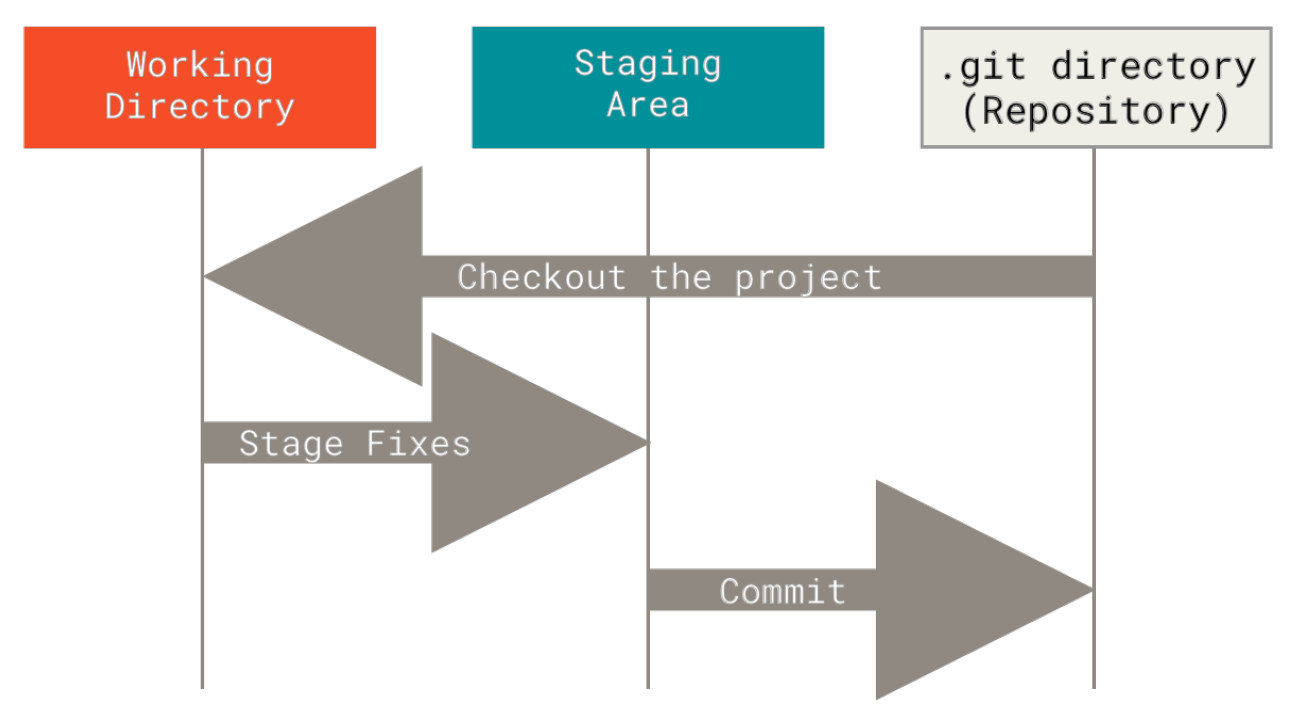
\includegraphics[width=15cm]{imagens/sections_git_project.png}
    \label{figura:secoes_projeto_git}
\end{figure}

